% TPI - Propuestas final de proyecto para el Trabajo Practico Integrador

\documentclass{article}

\usepackage{arxiv}

\usepackage[utf8]{inputenc} % allow utf-8 input
\usepackage[T1]{fontenc}    % use 8-bit T1 fonts
\usepackage[spanish]{babel}
\usepackage{hyperref}       % hyperlinks
\usepackage{url}            % simple URL typesetting
\usepackage{booktabs}       % professional-quality tables
\usepackage{amsfonts}       % blackboard math symbols
\usepackage{nicefrac}       % compact symbols for 1/2, etc.
\usepackage{microtype}      % microtypography
\usepackage{graphicx}
\usepackage{amsmath,amssymb}
\usepackage{float}
\usepackage{caption}
\usepackage{tikz}
\usetikzlibrary{arrows.meta}

\graphicspath{{figuras/}}

% Figuras generadas por src/02_figuras_propuesta.py a partir de los datos publicos.
\captionsetup{font=small,labelfont=bf,skip=6pt}

% Las figuras son anchas: sin esto LaTeX las manda a paginas propias y deja huecos.
\renewcommand{\topfraction}{0.88}
\renewcommand{\bottomfraction}{0.70}
\renewcommand{\textfraction}{0.12}
\renewcommand{\floatpagefraction}{0.80}

\raggedbottom

\title{Propuesta de TPI de Simulación: Evaluación del impacto de la Línea F sobre la operación de la red de Subte de la Ciudad de Buenos Aires}

\author{
  \textbf{Bruno Neirotti}\textsuperscript{1} \qquad \textbf{Alexis Galasco}\textsuperscript{2} \qquad \textbf{Salami Tomás}\textsuperscript{3} \qquad \textbf{Mesapelle Giani}\textsuperscript{4} \qquad \textbf{Lovatti Francisco}\textsuperscript{5} \\[0.5ex]
  \textsuperscript{1}Legajo: 47792 -- \texttt{bneirotti@gmail.com} \\
  \textsuperscript{2}Legajo: 51474 -- \texttt{alexis.galasco123@gmail.com} \\
  \textsuperscript{3}Legajo: 51534 -- \texttt{tomas.salami1@gmail.com} \\
  \textsuperscript{4}Legajo: 52897 -- \texttt{gianimesapelle04@gmail.com} \\
  \textsuperscript{5}Legajo: 52420 -- \texttt{franciscolovatti08@gmail.com} \\[0.5ex]
  Universidad Tecnológica Nacional -- FRRo \\
  Zeballos 1341, S2000, Argentina \\
}
\date{05 de agosto de 2026}

\begin{document}
\maketitle

% ---------- 1. Introducción ----------
\section{Introducción}

En este documento presentamos la propuesta que el grupo adopta para el Trabajo Práctico Integrador de la
materia Simulación. El trabajo aborda un problema de planificación: estimar, mediante simulación, qué
efecto tendría sobre el conjunto de la red de Subte de la Ciudad Autónoma de Buenos Aires la incorporación
de la futura Línea F.

El transporte público urbano guiado es la infraestructura que sostiene la movilidad cotidiana de las
ciudades densas, y a la vez es la más costosa y la menos reversible. Por esa razón, las decisiones de expansión
se apoyan habitualmente en modelos que permiten anticipar el desempeño de la red antes de que la obra
exista. La simulación de eventos discretos resulta apropiada para este tipo de evaluación porque
representa explícitamente los mecanismos que generan la congestión (llegadas de pasajeros variables en
el tiempo, intervalos irregulares entre formaciones, capacidad finita de coche y de andén, transbordos)
y permite comparar escenarios alternativos bajo los mismos supuestos, algo que un cálculo agregado de
capacidad no ofrece.

El criterio de selección del caso es la disponibilidad de datos. La demanda y la oferta de la red actual
están documentadas en registros públicos con marca de tiempo publicados por Subterráneos de Buenos Aires
(SBASE), de modo que las tasas de llegada y los intervalos de despacho se estiman a partir de mediciones y
no de supuestos propios. El escenario futuro tampoco es enteramente hipotético: la Línea F cuenta con traza
establecida por ley, se encuentra en proceso licitatorio y su Estudio de Impacto Ambiental fue sometido a
audiencia pública en agosto de 2026.

El expediente completo de esa evaluación ambiental fue obtenido
mediante pedido de vista ante la Agencia de Protección Ambiental y se incorpora a esta propuesta [13]: de él
provienen el trazado, las estaciones, las progresivas, las etapas constructivas y lo que resulta
decisivo para el modelo: los parámetros operativos con que la línea fue dimensionada. No obstante, ese
expediente no contiene una evaluación del efecto de la nueva línea sobre el conjunto de la red, que es
precisamente el objeto de este trabajo.

Los pedidos de acceso a la información pública para
obtener ese material se realizaron oportunamente a las autoridades gubernamentales correspondientes, conformando así los documentos presentes en el apartado de referencias de este documento.

% ---------- 2. Propuesta ----------
\section{Propuesta}

\subsection{Problema}

La red de Subte de Buenos Aires opera seis líneas con una demanda concentrada en dos picos diarios y muy
desigualmente repartida entre estaciones. A esa concentración temporal se suma una característica
estructural: el trazado es fuertemente radial, con líneas que convergen sobre el área central, de modo que
buena parte de los viajes entre el sur y el norte de la ciudad solo puede resolverse transbordando en el
macrocentro. El resultado son estaciones de combinación y tramos troncales que operan cerca de su
capacidad en hora pico, mientras otros sectores de la red circulan holgados.

\begin{figure}[!t]
  \centering
  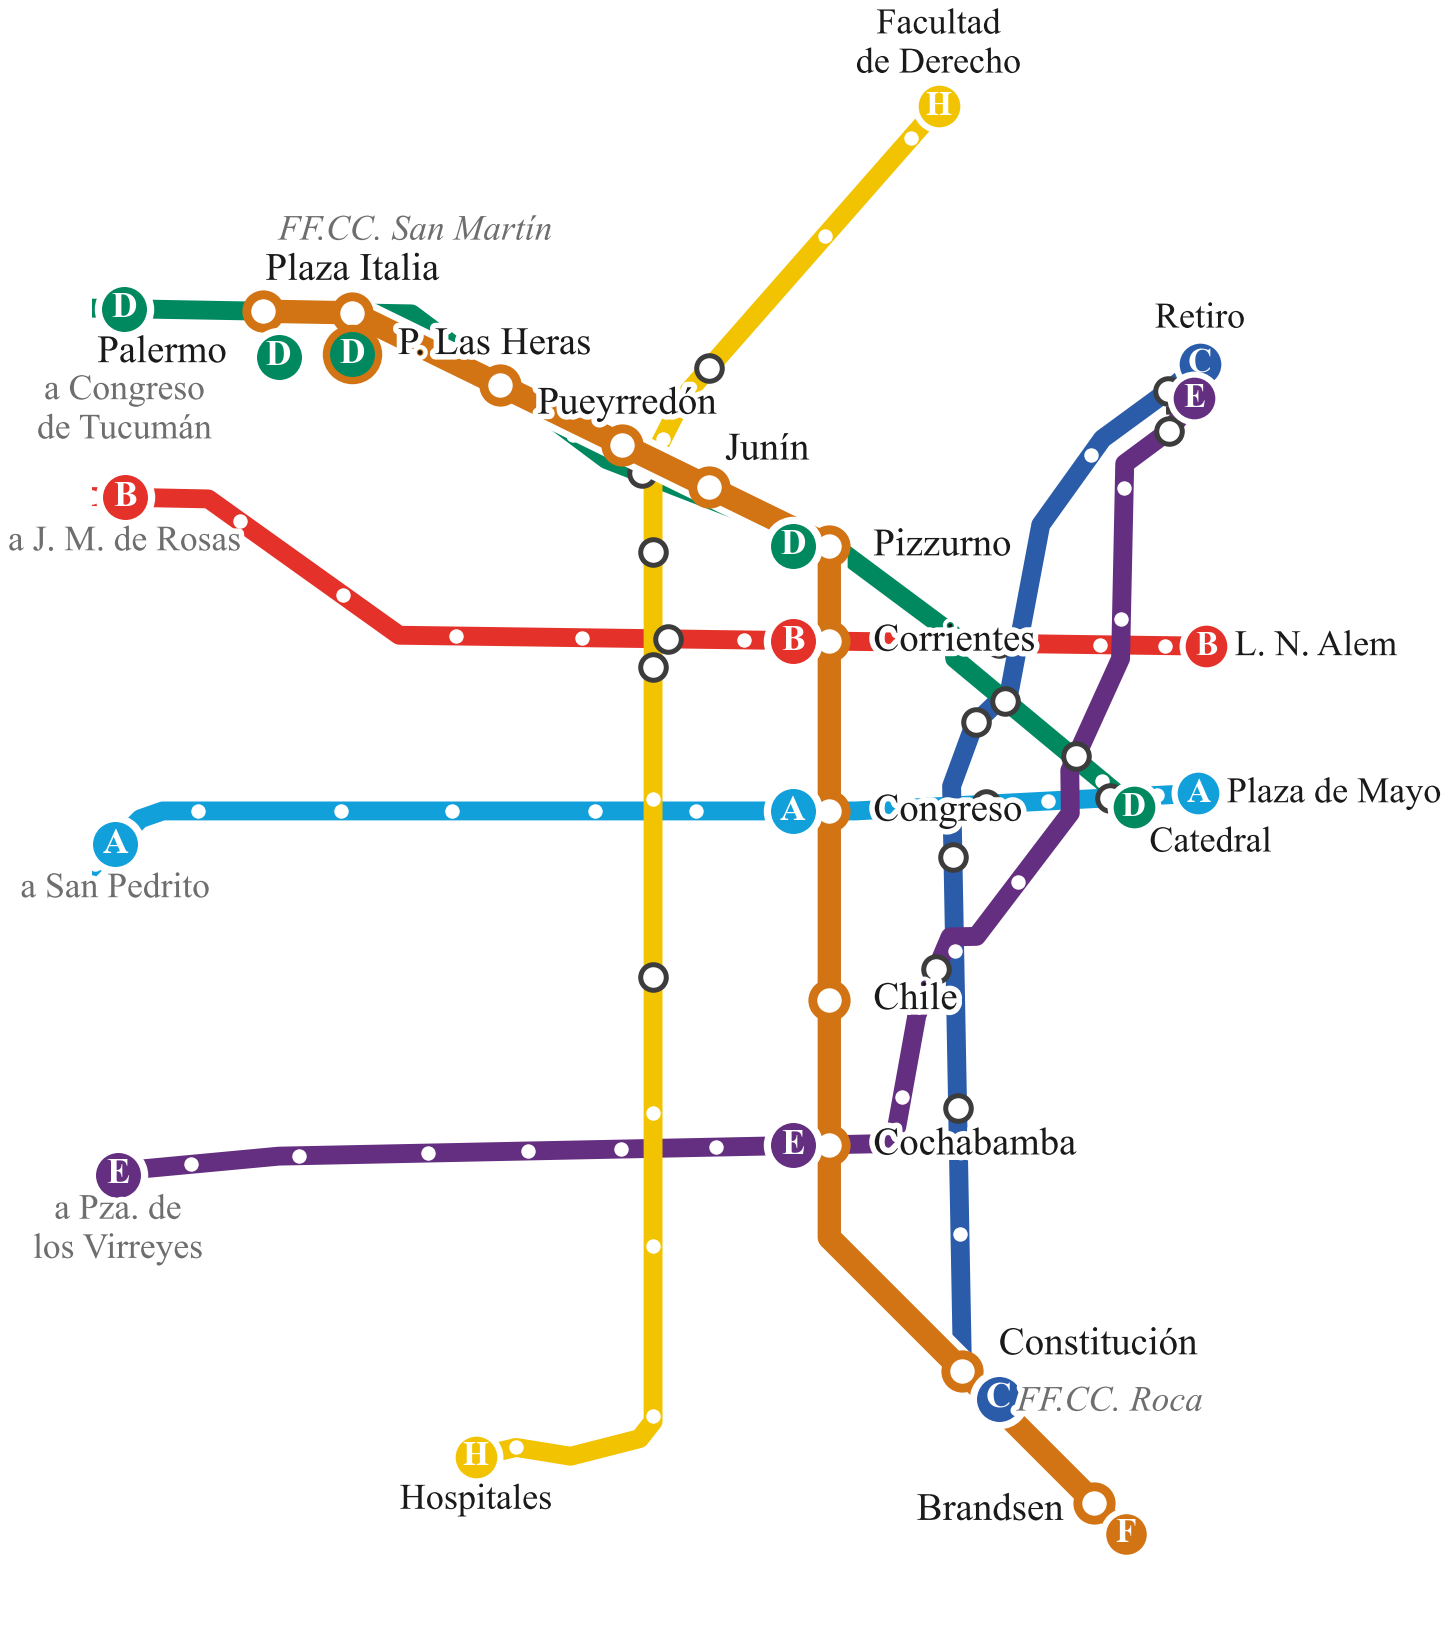
\includegraphics[width=0.88\linewidth]{red-y-linea-f.png}
  \caption{El área central de la red de Subte y el corredor de la Línea F, con sus doce estaciones. Es un
  diagrama topológico y no un mapa: no está a escala, y las líneas radiales se cortan en el borde de la
  vista indicando hacia qué cabecera continúan. El trazado de las seis líneas en operación se tomó del
  \textit{Mapa de red} oficial de SBASE [5] y el espaciado de sus estaciones, del feed GTFS [6]; la Línea F
  se ubicó anclándola en las estaciones con las que combina e interpolando las restantes según las
  progresivas del Estudio de Impacto Ambiental [13]. Junto a cada estación de la Línea F va el distintivo de
  la línea con la que combina: con anillo blanco, las seis que el Estudio declara estación por estación; con
  anillo naranja, las dos que solo figuran en el mapa oficial del proyecto [14] --- la Línea D en Plaza
  Italia y la Línea H en Pueyrredón, que el Estudio menciona sin precisar dónde. De esas ocho sale la cifra
  de estaciones de combinación que citan los anuncios y que el expediente ambiental no respalda.}
  \label{fig:red}
\end{figure}

La Línea F fue concebida precisamente como respuesta a ese desequilibrio. Su traza fue establecida por la
Ley 670 de la Ciudad [10], fue revisada en el Plan Estratégico y Técnico para la Expansión de la Red de
Subtes (PETERS) elaborado para SBASE con financiamiento del Banco Interamericano de Desarrollo [11], y hoy
forma parte
del proyecto \textit{Línea F -- Sistema Integrado de Movilidad}, bajo licitación pública nacional
e internacional y con audiencia pública ambiental. Se trata de un corredor
transversal entre Barracas y Palermo, con doce estaciones que vincularían las seis líneas existentes entre
sí y con los ferrocarriles Roca y San Martín, y cuya ejecución está prevista en dos tramos. En cuanto a su
magnitud, el pliego describe una línea de 9,8 km [12] y el Estudio
de Impacto Ambiental refiere 10,9 km de túneles [13]. El objetivo de descongestionar las líneas existentes y de mejorar la
conectividad norte--sur figura en la comunicación oficial del proyecto [14] y se reitera en el expediente
ambiental, donde el PETERS es citado como el estudio que plantea a la Línea F como la alternativa para que
la Línea C opere sin congestión con proyección de demanda a 2030 [13].

A lo anterior se le suma un dato del propio expediente que permite dimensionar el
mecanismo: el 70\,\% de los viajes que incluyen una etapa en la Línea C corresponde a combinaciones con el
ferrocarril, de modo que el alivio esperado depende de que la nueva línea capte la transferencia desde la
terminal Constitución. La comunicación oficial estima además una demanda de 270.000 a 300.000 pasajeros
diarios; si bien se trata de una cifra anunciada y no del resultado de un estudio publicado. El
presupuesto oficial de la obra asciende a 1.350 millones de dólares con anticipo financiero del 20\,\%, según
las Cláusulas Particulares del pliego y la resolución que postergó la apertura de ofertas [12].

La revisión del expediente ambiental completo
permite precisar qué falta y qué no. El expediente sí aporta el dimensionamiento de la nueva línea y un
perfil de carga por estación, sentido y hora pico elaborado para ella. En cambio, no contiene ninguna
comparación del funcionamiento de la red con y sin el proyecto, ni una matriz origen--destino de la red a
nivel de estación, ni parámetros operativos de las seis líneas existentes, ni cuantificación alguna del
alivio atribuido a las líneas C y D, que se enuncia únicamente en términos cualitativos. Los análisis con y
sin proyecto que el estudio incluye corresponden a microsimulaciones de tránsito de superficie durante la
etapa de obra, no a la operación de la red subterránea. Sigue sin estar disponible, entonces, una evaluación
desagregada que indique en qué estaciones, en qué tramos y en qué franjas horarias se produciría el alivio,
ni qué frecuencia de servicio sería necesaria para que ese alivio se materialice. Frente a una inversión de
esa magnitud y a un plazo de obra de varios años, resulta razonable disponer de un modelo que permita
comparar el desempeño de la red con y sin la nueva línea, y que además permita explorar distintos niveles de
frecuencia de la Línea F.

El problema, entonces, requiere representar la red
como un sistema conectado, en el que un viaje puede resolverse por distintos caminos y en el que la
aparición de una traza nueva modifica la elección de ruta de una parte de los pasajeros y, con ello, la
carga que soportan las líneas existentes. Ese planteo exige una matriz origen--destino [2], y ninguna fuente
pública la ofrece directamente: el registro de molinetes informa ingresos por estación pero no destinos, y
el dataset de viajes y etapas del Área Metropolitana, que sí informa destinos, corresponde a un único día
hábil típico y los obtiene por imputación. Reconciliar ambas fuentes y declarar de manera explícita los
supuestos que esa reconciliación introduce forma parte del problema a resolver.

\subsection{Objetivos}

\textbf{Objetivo general.} Construir un modelo de simulación de eventos discretos de la red de Subte de la
Ciudad Autónoma de Buenos Aires, calibrado con datos públicos de demanda y de oferta, que permita comparar
el desempeño operativo de la red actual con el de un escenario futuro que incorpore la Línea F.

\textbf{Objetivos específicos.}
\begin{itemize}
  \item Caracterizar la demanda de ingreso a cada estación por franja horaria y tipo de día a partir del
    registro de molinetes, y aprovechar la codificación de andén que ese registro contiene para
    contrastar el reparto entre andenes que el modelo produce.
  \item Construir una matriz origen--destino a nivel de estación, derivada de las etapas de subte del
    dataset de viajes y etapas del Área Metropolitana y escalada a los niveles de demanda medidos por
    los molinetes, dejando explícitos los supuestos que introduce esa combinación.
  \item Caracterizar el intervalo real entre formaciones despachadas y su dispersión por línea y franja
    horaria a partir del registro de trenes despachados, y contrastarlo con la frecuencia nominal
    programada.
  \item Implementar en AnyLogic un modelo de la red actual que incluya las seis líneas, sus estaciones y
    sus combinaciones, con una profundidad de calibración mayor en el corredor de la Línea F y en las
    líneas con las que combina, y validarlo contra un período no utilizado para el ajuste.
  \item Incorporar un escenario futuro con la Línea F, construido a partir de la traza, las estaciones y
    las combinaciones definidas en la documentación oficial del proyecto.
  \item Definir y medir un conjunto de indicadores operativos comparables entre escenarios.
  \item Comparar los escenarios considerados: red actual, red con la traza completa de la Línea F y
    variantes de frecuencia de la nueva línea.
  \item Analizar el efecto sobre la congestión y la redistribución de la demanda entre líneas, y evaluar
    la sensibilidad de los resultados a los supuestos declarados en la construcción de la matriz
    origen--destino.
\end{itemize}

\subsection{Metodología}

\textbf{Demanda.} La fuente principal es el dataset \textit{Subte: Viajes Molinetes} [3], publicado por
SBASE en Buenos Aires Data, con una fila por molinete, estación y bloque de quince minutos, discriminando
pasajeros pagos, con pase y franquiciados. De allí se estima la tasa de ingreso a cada estación por franja
horaria y tipo de día, agregando los molinetes de una misma estación. Sobre esta fuente pesa una
discontinuidad que condiciona la elección de períodos: la apertura a medios de pago distintos de SUBE (pago sin contacto desde diciembre de 2024 y código QR desde mayo de 2025) amplió la cobertura del registro, cambio que los archivos
publicados reflejan en su denominación. Los totales anteriores y posteriores a esa apertura no son
comparables en nivel, de modo que el ajuste y la validación se realizan dentro del régimen homogéneo
posterior.

\textbf{Oferta.} La operación real se caracteriza con el dataset \textit{Subte: Trenes despachados} [4],
que informa día, tipo de día, línea, cantidad de coches, hora de salida de cada cabecera y causa asociada a
cada formación despachada. De allí se reconstruye la serie de intervalos reales entre despachos sucesivos
por línea y franja, se separan los eventos con causa de demora registrada de la variabilidad propia de la
operación, y se obtiene la composición de las formaciones. La frecuencia nominal de contraste proviene del
\textit{Cronograma de servicio} y de \textit{Frecuencia del subte} [15], y la disponibilidad de material
rodante del recurso \textit{Estado de flota} incluido en [4].

\textbf{Topología y tiempos de recorrido.} La estructura física de la red se toma del feed
\textit{Subte: GTFS} [6], que aporta la secuencia ordenada de estaciones de cada línea y sentido, los
tiempos de llegada y salida del tren en cada estación (de los que se derivan el tiempo de recorrido de
cada tramo y el tiempo de detención en andén), las distancias acumuladas sobre la traza, la jerarquía
estación--andén--acceso y, en el archivo de transbordos, el tiempo mínimo de combinación medido para cada
par de andenes conectados. Esto reemplaza la estimación propia de esos parámetros. Las frecuencias programadas que el feed contiene son
previas a la pandemia (año 2019) y no se emplean, porque los intervalos de despacho se estiman del registro de
operación real [4]. La
georreferenciación de estaciones y accesos se complementa con \textit{Subte: Estaciones} [5] y
\textit{Bocas de Subte} [7]. El Premetro queda fuera del alcance del modelo.

\textbf{Matriz origen--destino.} Los destinos provienen del dataset \textit{Viajes y etapas en transporte
público del Área Metropolitana de Buenos Aires} [8], estimado a partir de registros SUBE; cada etapa de
subte informa origen, destino, línea de ascenso, hora y factor de expansión. Su documentación metodológica
[9] fija tres condiciones de uso. Los datos corresponden a un único día hábil típico de octubre o noviembre,
no a un promedio anual; se emplea la edición 2024. Las coordenadas publicadas no son la ubicación real de la
transacción sino el centroide del hexágono H3 de resolución 10 que la contiene, de unos 150 m de diámetro [16]. Sabiendo eso, verificamos que los 89 centroides distintos correspondientes a etapas de subte se ubican a una mediana de
44 m y a un máximo de 70 m de alguna estación del listado oficial [5], de modo que la correspondencia entre
celda y estación es unívoca y no constituye un supuesto de reparto.

Asimismo, los destinos no son observados sino
imputados por el organismo publicador bajo dos reglas declaradas: parada más cercana con tolerancia de
2,2 km, y simetría diaria del primer y último viaje. Un rasgo de esa imputación resulta determinante: las seis líneas se tratan como ramales de una sola, por lo
que toda estación puede ser origen y destino de cualquier otra.

La matriz es entonces estación--estación para el
conjunto de la red y ya contiene los viajes con combinación sin desagregar el camino recorrido, que es
exactamente lo que el modelo necesita: la ruta y los transbordos son resultado de la simulación y no un dato
de entrada, condición para que agregar la Línea F redistribuya la carga por sí misma.

El archivo aporta
587.980 etapas de subte, 740.675 una vez expandidas, de las cuales un 4,1\,\% pertenece a viajes con alguna
etapa sin destino imputado y se trata por separado. Restan dos ajustes propios, objeto del análisis de
sensibilidad: la matriz tiene resolución horaria, por lo que el perfil intrahorario se toma de los
molinetes, y su nivel absoluto se escala a los totales que estos miden. Este segundo ajuste no es menor: el
proceso de depuración del dataset descarta un 27,5\,\% de las transacciones originales por problemas de
geolocalización, de imputación o de registro, y el factor de expansión que compensa esa pérdida está topeado
en 3 para evitar que una línea con pérdida excesiva distorsione el resultado.

\textbf{Escenario futuro.} La configuración de la Línea F se toma de documentación oficial: la traza
establecida por la Ley 670 [10], el pliego de la licitación \textit{Ingeniería, construcción y equipamiento
Línea F} publicado en el portal BA Obras [12], el expediente del Estudio de Impacto Ambiental obtenido por
pedido de vista ante la Agencia de Protección Ambiental [13] y el PETERS [11] como antecedente de
planificación. El capítulo de descripción del proyecto del Estudio aporta el recorrido, las doce estaciones
proyectadas con sus progresivas sobre la traza, las combinaciones con las líneas existentes y la división en
tramos constructivos.

El Estudio dimensiona la línea con un intervalo entre
formaciones de 1,5 minutos (equivalente a cuarenta trenes por sentido y por hora), una capacidad de
1.075 pasajeros por formación y, en consecuencia, una capacidad de transporte de 43.000 pasajeros por
sentido y por hora; un tiempo de detención en estación de 30 segundos; velocidades de diseño de 90 km/h en
tramos rectos, reducidas a 70 y 45 km/h según la curvatura; aceleración de 1 m/s\textsuperscript{2} y
frenado de 1,1 m/s\textsuperscript{2}; y una flota necesaria de 25 formaciones. Prevé además andén central
en las doce estaciones y un recorrido peatonal de combinación no mayor a 100 m, valor que se adopta para el
tiempo de transbordo de las estaciones nuevas. Los tiempos de recorrido entre estaciones se derivan de las progresivas publicadas y de esos mismos parámetros cinemáticos. La frecuencia de
servicio se conserva como variable de escenario: el valor de 1,5 minutos es el de diseño y no
necesariamente el real, de modo que se lo toma como cota superior de oferta y se recorren
valores menores. El registro de despachos de las líneas en operación permite dimensionar cuán exigente es
ese valor de diseño. Medido en cabecera sobre los días hábiles típicos, el intervalo de la línea más
frecuente de la red actual en hora pico es el de la Línea C, con una mediana de 3,15 minutos entre
formaciones, equivalente a diecinueve trenes por sentido y por hora [4]: el intervalo previsto para la
Línea F supone despachar 2,1 veces más seguido que lo que hoy alcanza la mejor línea en servicio. El
supuesto no es inverosímil, tratándose de una línea nueva con señalamiento nuevo, pero es de magnitud
suficiente como para justificar que la frecuencia se trate como variable de escenario y no como dato, y
para que el rango recorrido en el análisis de sensibilidad se extienda hasta los valores efectivamente
observados en la red.

\textbf{Ajuste de distribuciones.} Las llegadas de pasajeros por estación y franja y los intervalos entre
formaciones se ajustan siguiendo el procedimiento visto en la carrera [1]: construcción de histogramas,
estimación de parámetros por máxima verosimilitud y pruebas de bondad de ajuste. La partición entre ajuste y
validación se hace por período, reservando datos no utilizados para estimar. Los dos registros admiten
particiones distintas y por razones distintas. El de despachos no se ve afectado por el cambio en los medios
de pago, de modo que su historia completa desde 2015 es homogénea y permite reservar un año entero. El de
molinetes sí lo está, por lo que ambos períodos deben pertenecer al régimen de cobertura posterior a
diciembre de 2024; la partición se realiza en ese tramo y se controla la estacionalidad comparando meses y
tipos de día equivalentes. Se deja constancia de que esta restricción reduce el margen temporal disponible
respecto de lo que la extensión de las series publicadas sugeriría, y de que es preferible asumirla antes
que validar contra un período cuya diferencia de nivel respondería a un cambio en el registro y no al
desempeño del modelo.

\textbf{Implementación en AnyLogic.} El modelo representa la red como un conjunto de líneas, cada una
compuesta por una secuencia de estaciones y tramos, vinculadas por estaciones de combinación a las que se
asocia el tiempo mínimo de transbordo que el GTFS declara para cada par de andenes. Los pasajeros se generan
en cada estación según la tasa ajustada para su franja horaria, reciben un destino sorteado a partir de la
matriz origen--destino y siguen una ruta tomada de una tabla de caminos mínimos precalculada fuera del
modelo, con una penalización por transbordo; no se implementan algoritmos de asignación dinámica. Las
formaciones se despachan desde cada cabecera según la distribución de intervalos ajustada sobre el registro
de despachos, recorren cada tramo con el tiempo derivado del GTFS y se detienen en cada estación durante el
tiempo de detención que ese mismo feed informa. El ascenso está limitado por la capacidad del coche: el
pasajero que no logra abordar permanece en el andén y espera la formación siguiente. El andén se modela como un espacio de
capacidad finita, lo que permite medir la aglomeración de plataforma además de la ocupación a bordo. El
escenario con Línea F se obtiene agregando la nueva línea a la topología y recalculando la tabla de
caminos mínimos con el mismo procedimiento, de modo que la redistribución de pasajeros resulta del cambio
de estructura de la red y no de un supuesto impuesto sobre cada línea.

\textbf{Verificación y validación.} La verificación se realiza comparando, en un caso degenerado sin
variabilidad en el intervalo de despacho ni en la demanda, la ocupación resultante contra el cálculo
analítico directo de pasajeros acumulados en un intervalo fijo, y controlando la conservación de entidades:
los pasajeros que ingresaron a lo largo de una corrida deben coincidir con la suma de los que llegaron a
destino, los que están a bordo y los que permanecen en andén al final del período simulado.

La validación se restringe a magnitudes efectivamente observables en los registros públicos, que son tres. La
primera es el ingreso de pasajeros por estación, franja de quince minutos y tipo de día, contrastado contra
el período de molinetes reservado. La segunda es el reparto de la demanda entre líneas, contrastado contra la
distribución de las etapas de subte del dataset de viajes y etapas [8], que es una fuente independiente
construida con otra metodología y sobre otro período. Corresponde señalar por qué el control agregado natural
no está disponible: el recurso oficial de total anual de pasajeros por línea [5] dejó de actualizarse en
septiembre de 2020, de modo que no cubre el régimen posterior a la apertura de medios de pago, que es el
único que este trabajo puede utilizar. La tercera surge de una propiedad del registro de molinetes que
conviene explicitar:
el identificador de cada molinete codifica el andén en el que está instalado, de modo que el ingreso queda
atribuido a un sentido de circulación. Esa atribución no es completa (sobre el año 2025 alcanza al
  70,5\,\% de los ingresos, porque una parte de los identificadores no incluye el campo de andén y hay
estaciones enteras sin él), y por eso la demanda se genera en el modelo a nivel de estación y no de andén,
evitando introducir un criterio de reparto para el resto. Pero el reparto entre andenes que el modelo produce
como resultado de la asignación de ruta sí puede contrastarse contra el observado en las estaciones que
cuentan con el dato. Es una validación parcial y sesgada por construcción, en tanto cubre solo un subconjunto
de estaciones que no fue elegido por nosotros.
Corresponde señalar una limitación de fondo: la ocupación a bordo y la aglomeración de plataforma, que son
indicadores centrales del trabajo, no se registran en ninguna fuente pública. Son salidas del modelo sin
contraparte empírica, dependientes de la matriz origen--destino y, por lo tanto, del supuesto de escalado
declarado más arriba. No se las valida y no se las presenta como magnitudes medidas, sino como resultados
condicionados a supuestos explícitos, cuya utilidad reside en la comparación entre escenarios evaluados bajo
esos mismos supuestos y no en términos absolutos.

Para el escenario futuro no existe, por definición, dato observable de ninguna clase, pero el expediente
ambiental aporta un término de comparación más exigente que el orden de magnitud de la cifra anunciada. El
Estudio publica, por cada una de las doce estaciones y para ambos sentidos, la cantidad de pasajeros que
suben, bajan y permanecen a bordo en la hora pico de la mañana y en la de la tarde, tomada de un análisis de
demanda elaborado por SBASE en 2019 [13]. De esas tablas se obtiene el perfil de carga por tramo. La carga por tramo que el modelo produzca para la Línea F se contrasta
contra ese perfil.

Ese contraste exige, sin embargo, una salvedad que surge de un control de consistencia entre fuentes
oficiales realizado sobre el registro de molinetes [3]. Los ascensos que el perfil de SBASE totaliza en la
hora pico, unos 73.900 sumando ambos sentidos, solo resultarían compatibles con la cifra anunciada de
270.000 a 300.000 pasajeros diarios si la Línea F concentrara alrededor del 25\,\% de su demanda diaria en
una sola hora. La red actual no exhibe esa concentración: medida sobre los días hábiles típicos de 2025 como
ventana móvil de sesenta minutos, la red concentra el 9,9\,\% de sus ingresos diarios en la hora pico y
ninguna de las seis líneas supera el 12,0\,\%. El contraste más directo disponible es Constitución, que es
el nodo de carga máxima de la Línea F según el perfil y que hoy ya existe como estación de la Línea C
alimentada por el mismo ferrocarril Roca: recibe 57.010 ingresos diarios y concentra el 17,5\,\% de ellos
en su hora pico, unos 9.950 ingresos, frente a los 32.640 ascensos en un solo sentido que el perfil proyecta
para la estación homónima de la Línea F. Los transbordos provenientes del ferrocarril atraviesan molinete,
de modo que la comparación no subestima la demanda de origen ferroviario.

Las dos cifras oficiales disponibles sobre la demanda de la Línea F no son conciliables entre sí. Si la
línea se comportara como la red actual, su perfil de hora pico implicaría del orden de 743.000 pasajeros
diarios, entre dos y tres veces la cifra anunciada; ese valor es una cota superior, porque los ascensos del
perfil incluyen los transbordos desde las otras seis líneas mientras que los molinetes registran únicamente
ingresos a la red. Si en cambio la cifra anunciada fuese correcta, la línea debería concentrar dos veces y
media lo que concentra la red existente. Al menos una de las dos es incorrecta y el trabajo no dispone de
información para determinar cuál. La consecuencia metodológica es doble: la cifra diaria anunciada no se
incorpora como insumo del modelo, criterio que ya se venía aplicando, y el perfil de SBASE se conserva como
contraste declarado, ahora con la salvedad expresa de que el nivel de concentración horaria que supone no
tiene correlato en la red en operación.

Cada escenario se corre con un mínimo de diez replicaciones, descartando el período de calentamiento, y los
resultados se informan con intervalos de confianza.

\begin{figure}[htbp]
  \centering
  \hyphenpenalty=10000\relax   % las cajas son angostas: partir palabras las afea
  \begin{tikzpicture}[
    font=\scriptsize,
    fuente/.style    ={draw=black!40, fill=black!6, rounded corners=1.5pt, text width=2.5cm,
                       align=center, inner sep=3pt, minimum height=1.05cm},
    insumo/.style    ={draw=black!55, fill=white, rounded corners=1.5pt, text width=2.5cm,
                       align=center, inner sep=3pt, minimum height=1.35cm},
    marco/.style     ={draw=black!70, fill=black!3, rounded corners=3pt},
    escenario/.style ={draw=black!55, fill=white, rounded corners=1.5pt, text width=4.1cm,
                       align=center, inner sep=3pt, minimum height=0.9cm},
    salida/.style    ={draw=black!70, fill=black!6, rounded corners=1.5pt, text width=13.4cm,
                       align=center, inner sep=4pt},
    fl/.style        ={-{Stealth[length=3.2pt,width=2.6pt]}, draw=black!55, line width=0.45pt}
  ]

  % --- fuentes públicas --------------------------------------------------
  \node[fuente] (f1) at ( 0.0, 0) {Molinetes [3]\\[1pt] ingresos por estación cada 15 min};
  \node[fuente] (f2) at ( 2.9, 0) {Trenes despachados [4]\\[1pt] salidas de cabecera};
  \node[fuente] (f3) at ( 5.8, 0) {GTFS [6]\\[1pt] topología y tiempos};
  \node[fuente] (f4) at ( 8.7, 0) {Viajes y etapas AMBA [8]\\[1pt] origen y destino};
  \node[fuente] (f5) at (11.6, 0) {Expediente del EsIA [13]\\[1pt] Línea F};

  % --- insumos del modelo ------------------------------------------------
  \node[insumo] (p1) at ( 0.0, -1.95) {Tasa de ingreso por estación, franja y tipo de día};
  \node[insumo] (p2) at ( 2.9, -1.95) {Distribución de intervalos reales entre despachos};
  \node[insumo] (p3) at ( 5.8, -1.95) {Grafo de la red: tramos, detenciones y transbordos};
  \node[insumo] (p4) at ( 8.7, -1.95) {Matriz origen--destino estación a estación};
  \node[insumo] (p5) at (11.6, -1.95) {Traza, progresivas y parámetros operativos};

  \foreach \i in {1,...,5} \draw[fl] (f\i.south) -- (p\i.north);

  % --- modelo y escenarios -----------------------------------------------
  \node[marco, minimum width=14.4cm, minimum height=2.25cm] (mod) at (5.8, -4.65) {};
  \node[anchor=north, inner sep=4pt] at (mod.north)
    {\textbf{Modelo de simulación de eventos discretos (AnyLogic)}};
  \node[escenario] (e1) at (3.1, -5.05) {Escenario base:\\ red actual};
  \node[escenario] (e2) at (8.5, -5.05) {Escenario futuro:\\ red con Línea F};
  \draw[fl] (e1.east) -- (e2.west);

  \foreach \i in {1,...,4} \draw[fl] (p\i.south) -- (p\i.south |- mod.north);
  \draw[fl] (p5.south) -- (e2.north east);

  % --- salida -------------------------------------------------------------
  \node[salida] (out) at (5.8, -6.85)
    {Indicadores comparables entre escenarios: espera en andén, tiempo de viaje,
     ocupación de coche por tramo, aglomeración de plataforma y pasajeros que no abordan};
  \draw[fl] (mod.south) -- (out.north);

  \end{tikzpicture}
  \caption{Esquema de la metodología. Cada fuente pública alimenta un insumo distinto del modelo y los
  números entre corchetes remiten a las referencias. El escenario futuro no se parametriza por separado: se
  obtiene agregando la Línea F a la topología del escenario base y recalculando la tabla de caminos mínimos,
  de modo que la redistribución de la demanda entre líneas es un resultado de la simulación y no un dato de
  entrada.}
  \label{fig:metodo}
\end{figure}

\subsection{Resultados esperados}

Esperamos obtener, en primer lugar, un cuadro comparativo de indicadores operativos entre el escenario
actual y los escenarios con Línea F: tiempo medio de espera en andén por estación y franja horaria, tiempo
medio de viaje completo dentro del sistema incluyendo transbordos, ocupación media y máxima de coche por
tramo, nivel de aglomeración de plataforma y proporción de pasajeros que no logran abordar la primera
formación que arriba.

En segundo lugar, esperamos caracterizar el uso de la nueva infraestructura: viajes diarios captados por la
Línea F, carga por tramo, tramo de máxima demanda y factor de ocupación resultante para la frecuencia
supuesta, junto con la variación de carga que se produce en cada una de las líneas existentes y en las
estaciones de combinación del área central. Eso permite identificar qué líneas y qué estaciones concentran
el beneficio y en qué franjas horarias se manifiesta, distinguiendo el alivio efectivo de la simple
redistribución de la congestión hacia otras combinaciones.

En tercer lugar, esperamos cuantificar cómo cambian esos resultados frente a los supuestos declarados:
cuánto varía el beneficio estimado según el criterio con que la matriz se escala a los niveles medidos y
según el tratamiento de las etapas sin destino imputado, y qué frecuencia mínima de la Línea F es necesaria
para que la mejora sea perceptible en los indicadores de la red.

No se considera un escenario de habilitación parcial de la línea. Aunque el Estudio de Impacto Ambiental
divide la obra en dos tramos constructivos, el Ministerio de Movilidad e Infraestructura informó que la
Línea F ``se desarrollara en UNA (1) única Etapa, desde Brandsen a Palermo / Pacífico'' y que, por la
metodología constructiva mediante tuneladora, ``no se prevé en principio la habilitación parcial de
funcionamiento de la Línea F antes de la finalización completa de las obras'' [17]. La partición en tramos
es entonces constructiva y no de puesta en servicio, de modo que el único escenario futuro con sentido
operativo es la traza completa.

En cuanto al alcance, el presente trabajo no pretende producir una previsión de demanda ni sustituir los
estudios oficiales del proyecto. Lo informativo es la comparación entre escenarios evaluados bajo esos
mismos supuestos, expresada en las magnitudes con las que se discute el nivel de servicio: minutos de
espera, minutos de viaje y pasajeros por coche.

% ---------- Referencias ----------
\section*{Referencias}
\begin{list}{}{\leftmargin=2em \itemindent=-2em \itemsep=0.25em}

\item[] [1] Law, A. M. (2015). \textit{Simulation Modeling and Analysis} (5.\textsuperscript{a} ed.).
  McGraw-Hill Education.

\item[] [2] Ortúzar, J. de D. y Willumsen, L. G. (2011). \textit{Modelling Transport} (4.\textsuperscript{a}
  ed.). John Wiley \& Sons.

\item[] [3] Subterráneos de Buenos Aires (SBASE). \textit{Subte: Viajes Molinetes}. Buenos Aires Data.
  Archivos anuales comprimidos, 2013--2025. Desde diciembre de 2024 se publican con la denominación
  \texttt{INCLUYEOTROMODOSDEPAGO}, que indica la incorporación de medios de pago distintos de la tarjeta SUBE.
  \url{https://data.buenosaires.gob.ar/dataset/subte-viajes-molinetes}

\item[] [4] Subterráneos de Buenos Aires (SBASE). \textit{Subte: Trenes despachados}. Buenos Aires Data.
  Recursos \textit{Formaciones despachadas -- Total} (CSV, 2015 a la actualidad) y \textit{Estado de flota}.
  \url{https://data.buenosaires.gob.ar/dataset/subte-trenes-despachados}

\item[] [5] Subterráneos de Buenos Aires (SBASE). \textit{Subte: Estaciones}. Buenos Aires Data. Incluye los
  recursos \textit{Estaciones de Subte}, \textit{Líneas de Subte} y \textit{Total de pasajeros de cada línea
  de subte por año}. Pese a que el título de este último indica ``desde junio 2013'', el archivo publicado
  abarca hasta 2020 y su última modificación registrada es del 7 de septiembre de 2020.
  \url{https://data.buenosaires.gob.ar/dataset/subte-estaciones}

\item[] [6] Subterráneos de Buenos Aires (SBASE). \textit{Subte: GTFS}. Buenos Aires Data. Feed versión 2.0;
  período declarado en \texttt{feed\_info} hasta el 31/12/2019 y calendario de servicios hasta el 31/12/2021.
  El portal advierte que los datasets en formato API y GTFS están suspendidos y en revisión.
  \url{https://data.buenosaires.gob.ar/dataset/subte-gtfs}

\item[] [7] Subterráneos de Buenos Aires (SBASE). \textit{Bocas de Subte}. Buenos Aires Data.
  \url{https://data.buenosaires.gob.ar/dataset/bocas-subte}

\item[] [8] Subsecretaría de Planificación de la Movilidad y Seguridad Vial. \textit{Viajes y etapas en
  transporte público del Área Metropolitana de Buenos Aires 2019 a 2024}. Buenos Aires Data.
  \url{https://data.buenosaires.gob.ar/dataset/viajes-etapas-transporte-publico}

\item[] [9] Observatorio de Movilidad y Seguridad Vial de la Ciudad de Buenos Aires, Ministerio de
  Infraestructura. \textit{Dataset de Viajes y Etapas en Transporte Público del Área Metropolitana de Buenos
  Aires. Notas para su uso, 2019--2025}. Abril de 2025. Documento metodológico del dataset [8].

\item[] [10] Legislatura de la Ciudad Autónoma de Buenos Aires. \textit{Ley 670}, sancionada el 8 de
  noviembre de 2001, de construcción de las líneas de subterráneos F, G e I, y sus modificatorias.
  \url{http://www2.cedom.gob.ar/es/legislacion/normas/leyes/ley670.html}

\item[] [11] Subterráneos de Buenos Aires (SBASE) y Banco Interamericano de Desarrollo. \textit{Plan
  Estratégico y Técnico para la Expansión de la Red de Subtes de Buenos Aires (PETERS)}. Estudio elaborado
  por AC\&A, publicado por SBASE, 2015.

\item[] [12] Gobierno de la Ciudad Autónoma de Buenos Aires, Ministerio de Movilidad e Infraestructura.
  \textit{Licitación pública nacional e internacional de etapa múltiple N.\textsuperscript{o}
  10241-0094-LPU25, ``Ingeniería, construcción y equipamiento línea de Subterráneo F''}. Expedientes
  EX-2025-43875108-GCABA-SSPO y EX-2025-43793855-GCABA-DGTALMI. Portal BA Obras. Se citan en particular el
  Pliego de Cláusulas Particulares PLIEG-2026-30055586-SSPO, el Pliego de Especificaciones Técnicas Rev. 01
  PLIEG-2026-30055895-GCABA-SSPO, los informes LF-GL-GEN-GNR-IN-003 y LF-GL-GEN-GNR-IN-004
  (\textit{Demandas Etapa I y II --- Medios de Salida}), y la Resolución N.\textsuperscript{o}
  175/GCABA-MMIGC/26, que posterga la apertura de ofertas al 10 de septiembre de 2026 y consigna el
  presupuesto oficial.
  \url{https://buenosairesobras.dguiaf-gcba.gov.ar}

\item[] [13] Agencia de Protección Ambiental, Gobierno de la Ciudad Autónoma de Buenos Aires.
  \textit{Estudio de Impacto Ambiental --- Proyecto ``Línea F -- Sistema Integrado de Movilidad, CABA''}.
  Expediente EX-2026-20211143-GCABA-APRA, 98 documentos, obtenido por pedido de vista. Estudio elaborado por
  Serman \& asociados s.a. Convocado a audiencia pública por Resolución N.\textsuperscript{o}
  195/GCABA-APRA/26, celebrada el 18 de agosto de 2026. Se citan en particular: IF-2026-20219129-GCABA-APRA,
  capítulo 3, \textit{Descripción del proyecto} --- parámetros operativos (p. 15), estimaciones de demanda por
  estación (pp. 15--16), estaciones y progresivas (pp. 20--21), cocheras y flota (p. 42), cronograma de obra
  (p. 100) ---; IF-2026-20220749-GCABA-APRA, capítulo 6, \textit{Estudios especiales} --- Línea C y PETERS
  (p. 62), pasajeros por estación (p. 97) ---; IF-2026-23674238-GCABA-DGDPM, intervención de la Dirección
  General de Diseño y Planificación de la Movilidad; e IF-2026-28526299-GCABA-DGPRO, \textit{Documento de
  divulgación}. Las estimaciones de demanda que el Estudio reproduce se atribuyen en él al
  \textit{Análisis de Demanda Línea F} elaborado por SBASE en 2019, documento que el expediente cita pero no
  incorpora.

\item[] [14] Gobierno de la Ciudad Autónoma de Buenos Aires. \textit{Anuncio del proyecto de construcción de
  la línea F de subte: trazado, estaciones, etapas y cronograma previsto}.
  \url{https://buenosaires.gob.ar/noticias/jorge-macri-anuncio-la-construccion-de-la-linea-f-de-subte}

\item[] [15] Subterráneos de Buenos Aires (SBASE). \textit{Subte: Cronograma de servicio} y
  \textit{Frecuencia del subte}. Buenos Aires Data.
  \url{https://data.buenosaires.gob.ar/dataset/subte-cronograma-servicio} y
  \url{https://data.buenosaires.gob.ar/dataset/frecuencia-subte}

\item[] [16] Uber Technologies y comunidad H3. \textit{H3: Hexagonal hierarchical geospatial indexing
  system}. Documentación oficial. \url{https://h3geo.org/docs}

\item[] [17] Gobierno de la Ciudad Autónoma de Buenos Aires. \textit{Respuesta a la Solicitud de Acceso a la
  Información Pública --- Ley 104, Contacto N.\textsuperscript{o} 00866317/26}. Expediente
  EX-2026-35399949-GCABA-DGAIGA. Se citan en particular: IF-2026-38553261-GCABA-SBASE, Subterráneos de Buenos
  Aires S.E., 26 de agosto de 2026 --- matriz origen--destino de la red a nivel de estación para día hábil,
  hora pico mañana y hora pico tarde, y perfiles de carga por tramo de las seis líneas, elaborados por EMOVA
  S.A. sobre transacciones SUBE de septiembre de 2024 ---; IF-2026-37530623-GCABA-MMIGC, Ministerio de
  Movilidad e Infraestructura, 20 de agosto de 2026 --- distancias entre estaciones proyectadas de la Línea F,
  intervalo de diseño, tiempo de viaje entre cabeceras, composición de las formaciones y etapas de
  habilitación ---; e IF-2026-38751180-GCABA-DGDPM, Dirección General de Diseño y Planificación de la
  Movilidad, 27 de agosto de 2026.

\end{list}

\end{document}
